\subsection{Resultate}

Praxisruf wurde wie in Kapitel 5 beschrieben erweitert.
Es wurde eine native iOS App entwickelt, welche den Funktionsumgang des bestehenden Mobile Clients vollständig unterstützt.
Weiter wurde mit AWS Polly ein Sprachsynthese Provider an das System angebunden.
Diese Anbindung wird verwendet, um bei Bedarf den Inhalt empfangener Benachrichtigungen automatisch vorlesen zu lassen.
Letztlich wurde WebRTC verwendet, um eine konfigurierbare Gegensprechanalge zu implementieren.

\clearpage

\subsubsection{Nativer Mobile Client}

Dieses Kapitel zeigt die umgesetzten Ansichten des Mobile Clients.

\subsubsection*{Anmeldung und Konfiguration}

Der Mobile Client bietet eine einfaches Verfahren zur Anmeldung und Konfiguration.
In einem ersten Schritt gibt der Praxismitarbeitende Benutzername und Passwort ein.
Anschliessend kann er auf einer zweiten Ansicht, die gewünschte Zimmerkonfiguration wählen.
Benutzer und Zimmerkonfiguration werden dabei gespeichert.
Bis sich der Benutzer manuell abmeldet wird bei allen zukünftigen Starts der App die gespeicherte Kombination von Benutzer und Zimmerkonfiguration wiederverwendet.

\begin{figure}[h]
    \centering
    \begin{minipage}[b]{0.4\textwidth}
        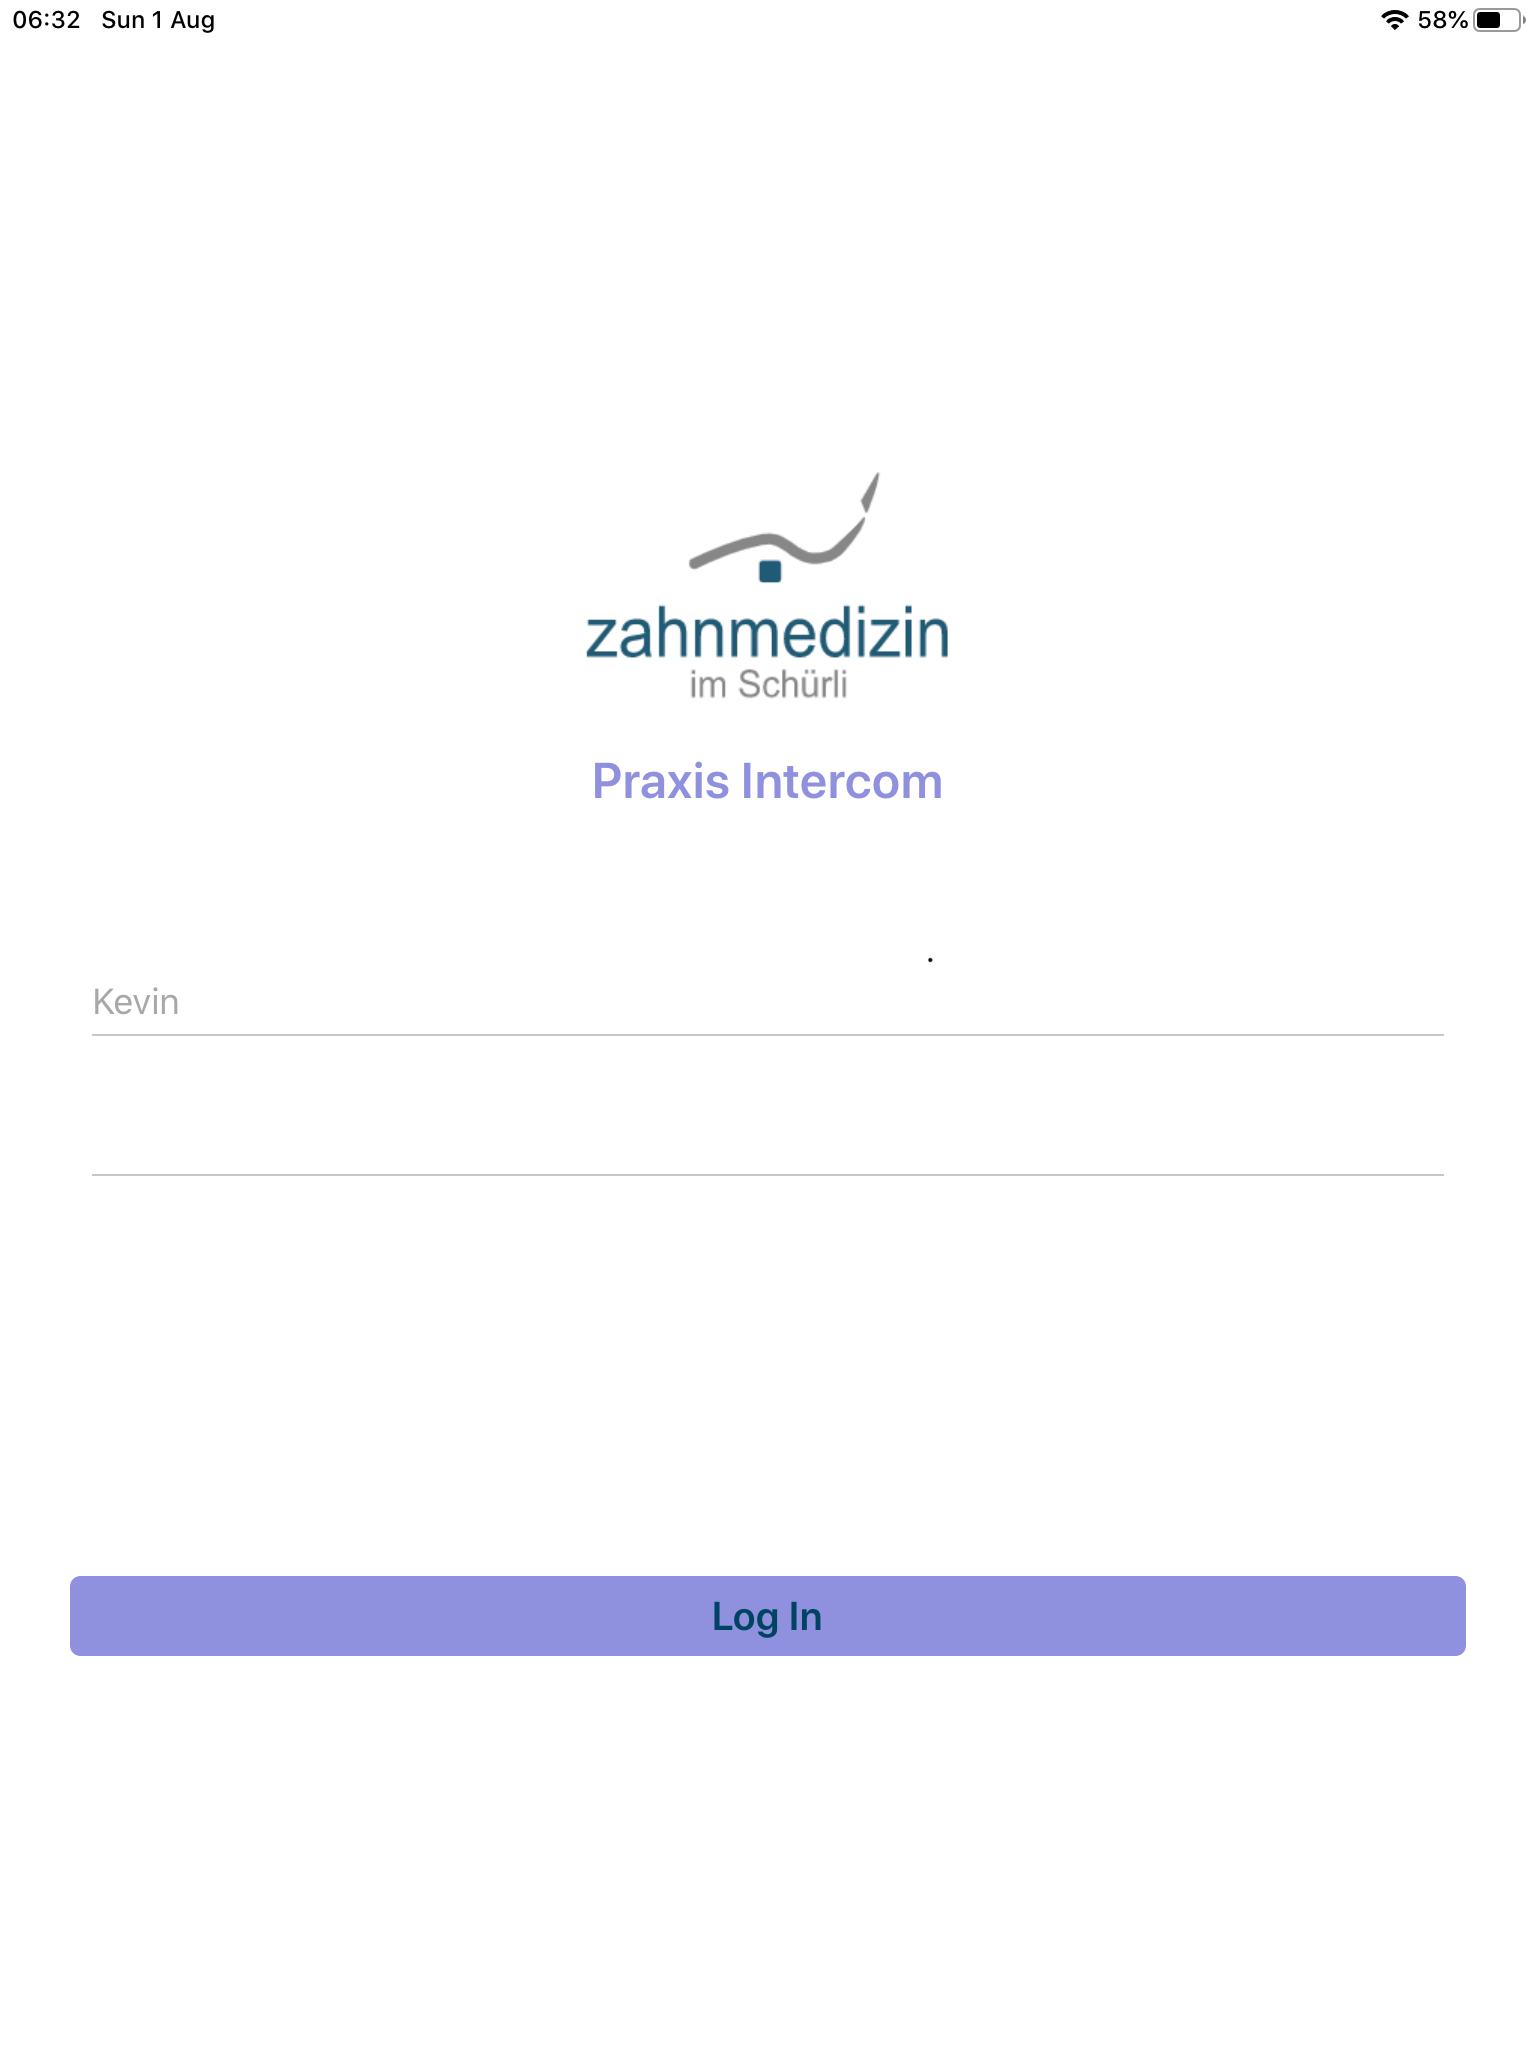
\includegraphics[width=\textwidth]{graphics/screenshots/placeholder}
        \caption{Ansicht Login}
    \end{minipage}
    \hfill
    \begin{minipage}[b]{0.4\textwidth}
        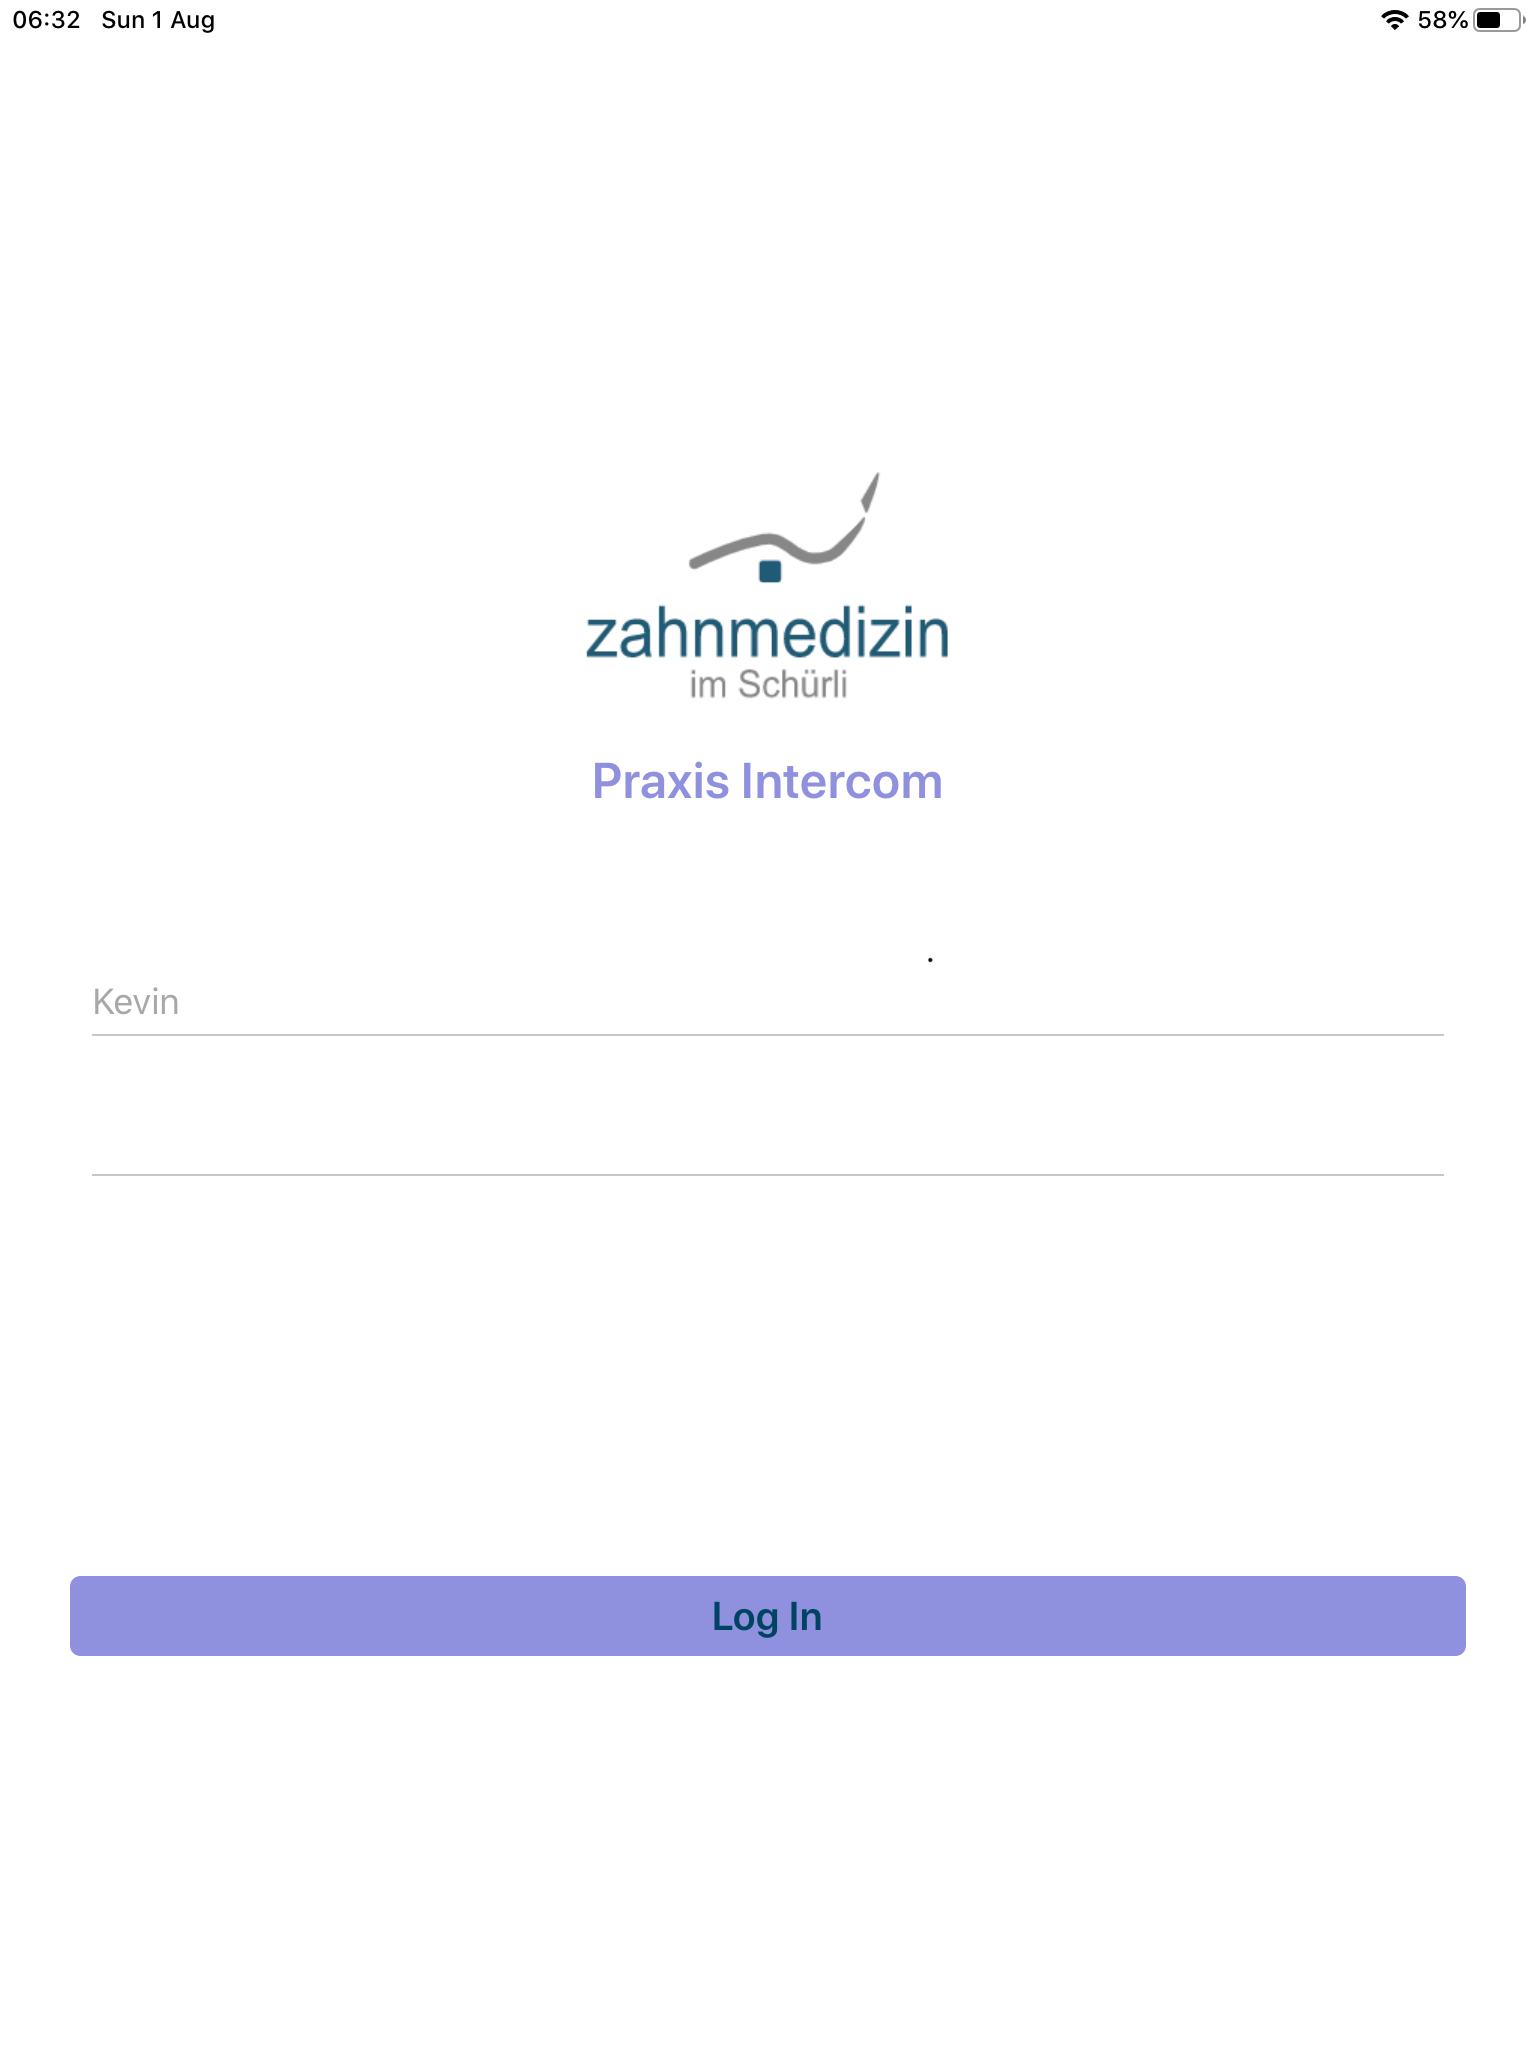
\includegraphics[width=\textwidth]{graphics/screenshots/placeholder}
        \caption{Ansicht Zimmerkonfiguration}
    \end{minipage}
    \label{fig:MobileClient-Screens1}
\end{figure}

\clearpage

\subsubsection*{Startseite und Inbox}

Nach der Anmeldung und Konfigurationsauswahl wird der Benutzer auf die Hauptansicht der App weitergeleitet.
Über eine Navigationsleiste am unteren Bildschirmrand kann zwischen den Bereichen Home, Inbox und Einstellungen
Der Bereich Home ist in zwei Teile gegliedert und beinhaltet Buttons über welche Benachrichtigungen versendet und Sprachverbindungen gestartet werden können.
Welche Buttons zur Verfügung stehen werden durch die gewählte Zimmerkonfiguration vorgegeben und wurden im Vorfeld vom Praxisadministrator konfiguriert.
Der Bereich Inbox zeigt eine Liste von empfangenen Benachrichtigungen sowie verpassten und vergangenen Anrufen.
Einträge in dieser Liste können durch eine Wischgeste (Swipe right) entfernt werden.

\begin{figure}[h]
    \centering
    \begin{minipage}[b]{0.4\textwidth}
        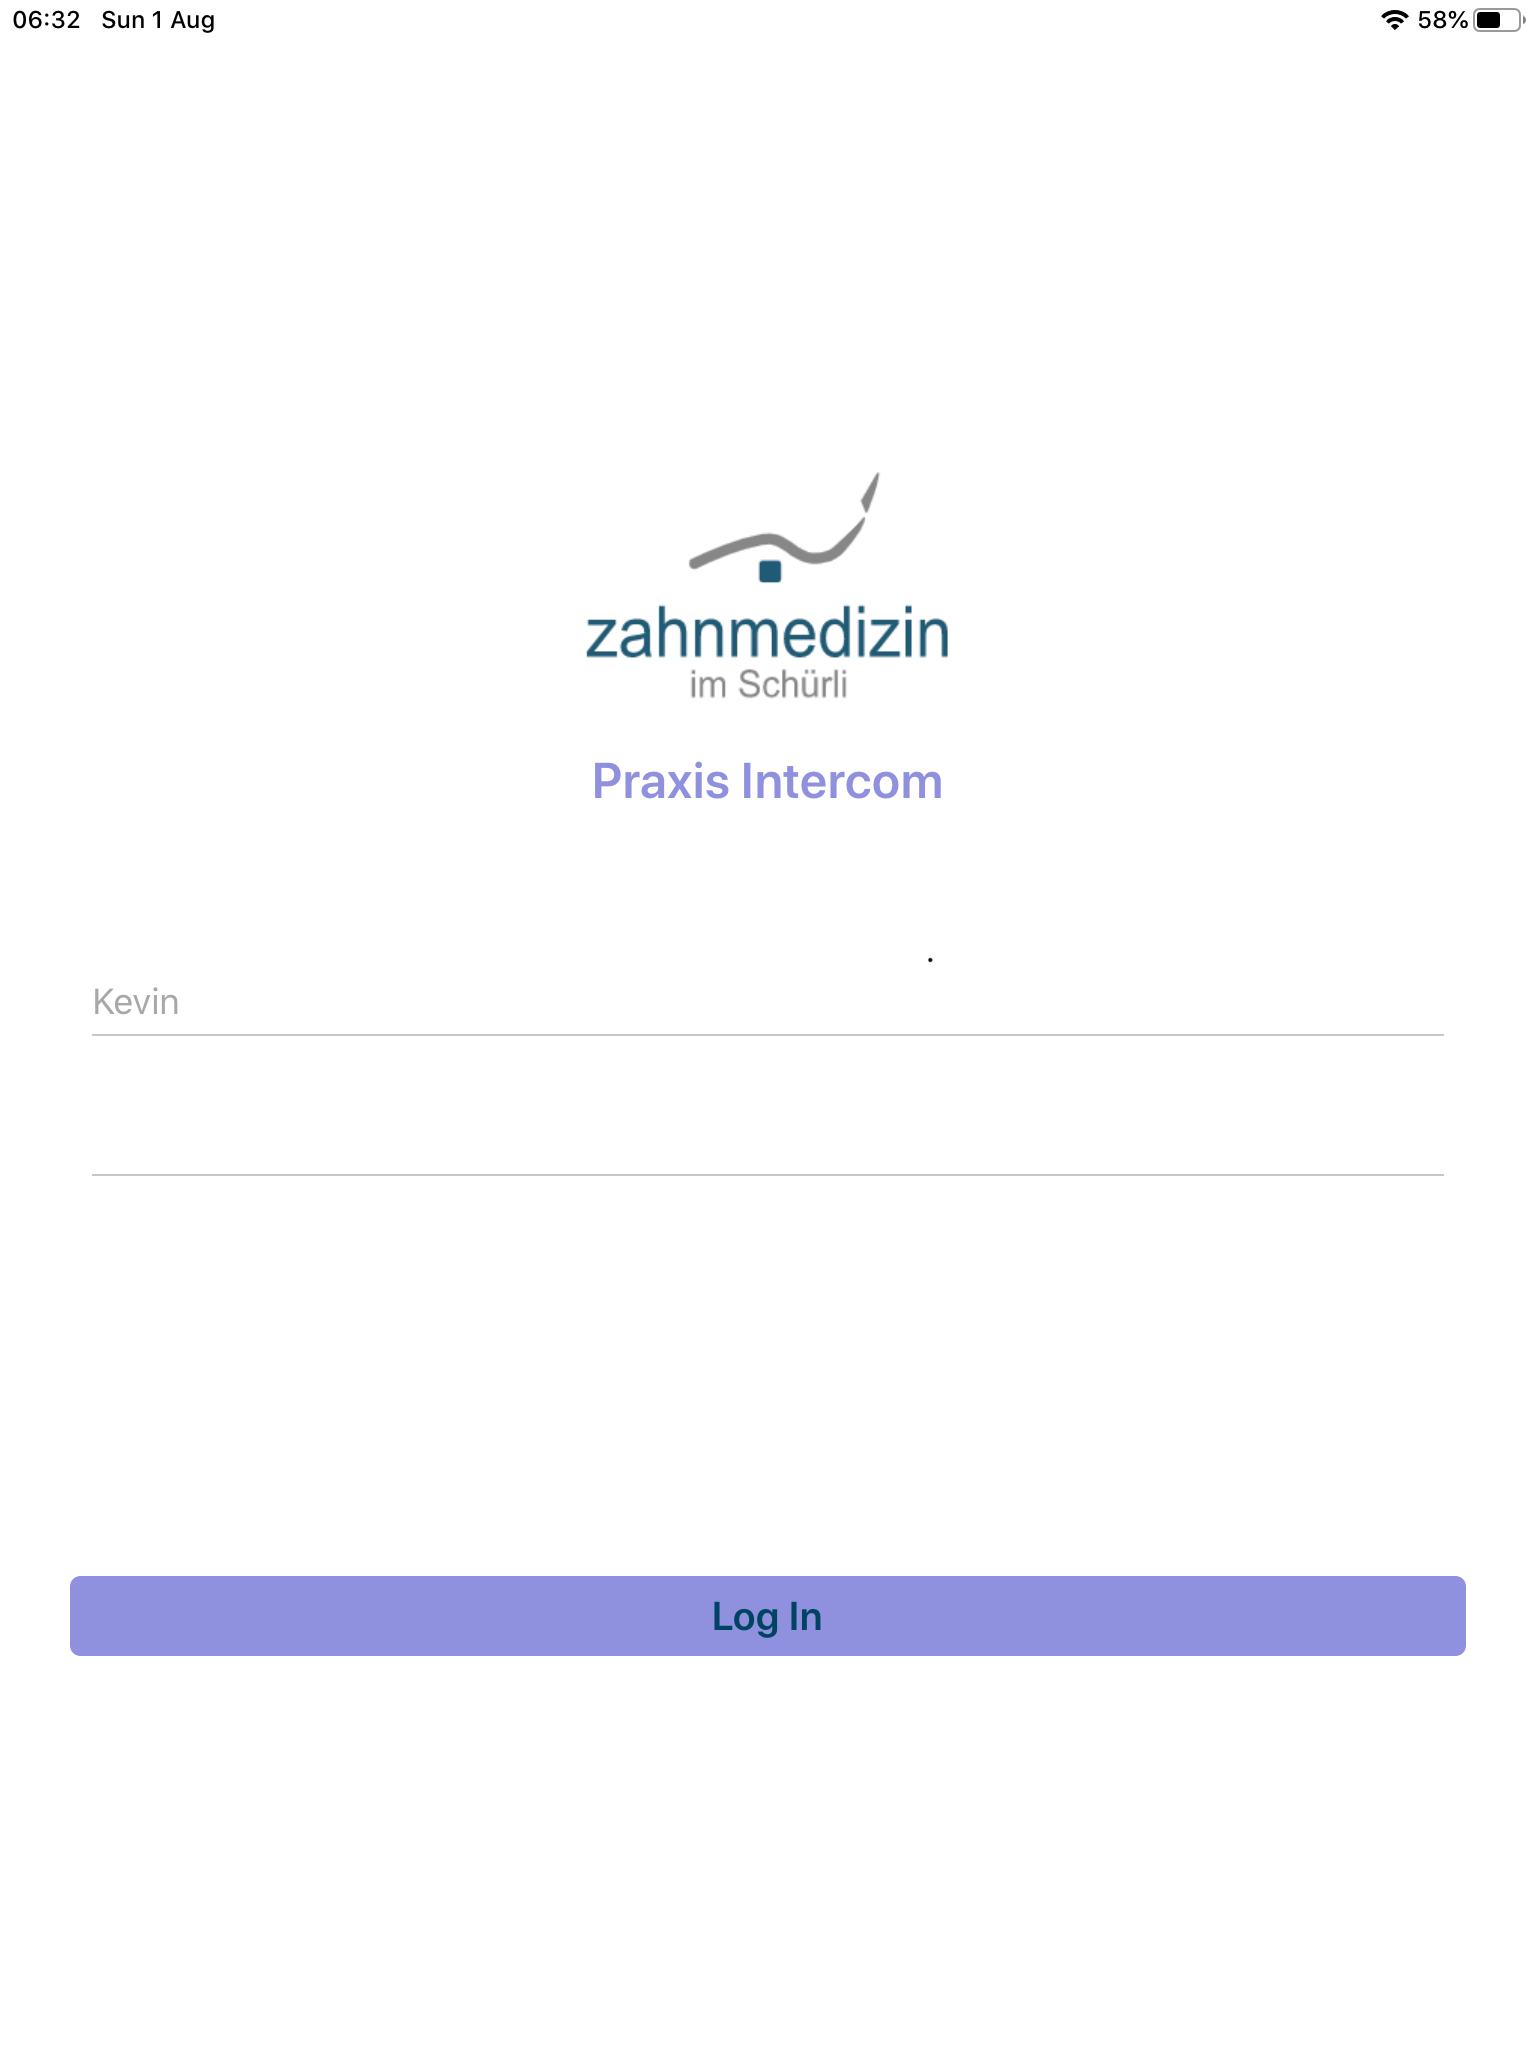
\includegraphics[width=\textwidth]{graphics/screenshots/placeholder}
        \caption{Ansicht Home}
    \end{minipage}
    \hfill
    \begin{minipage}[b]{0.4\textwidth}
        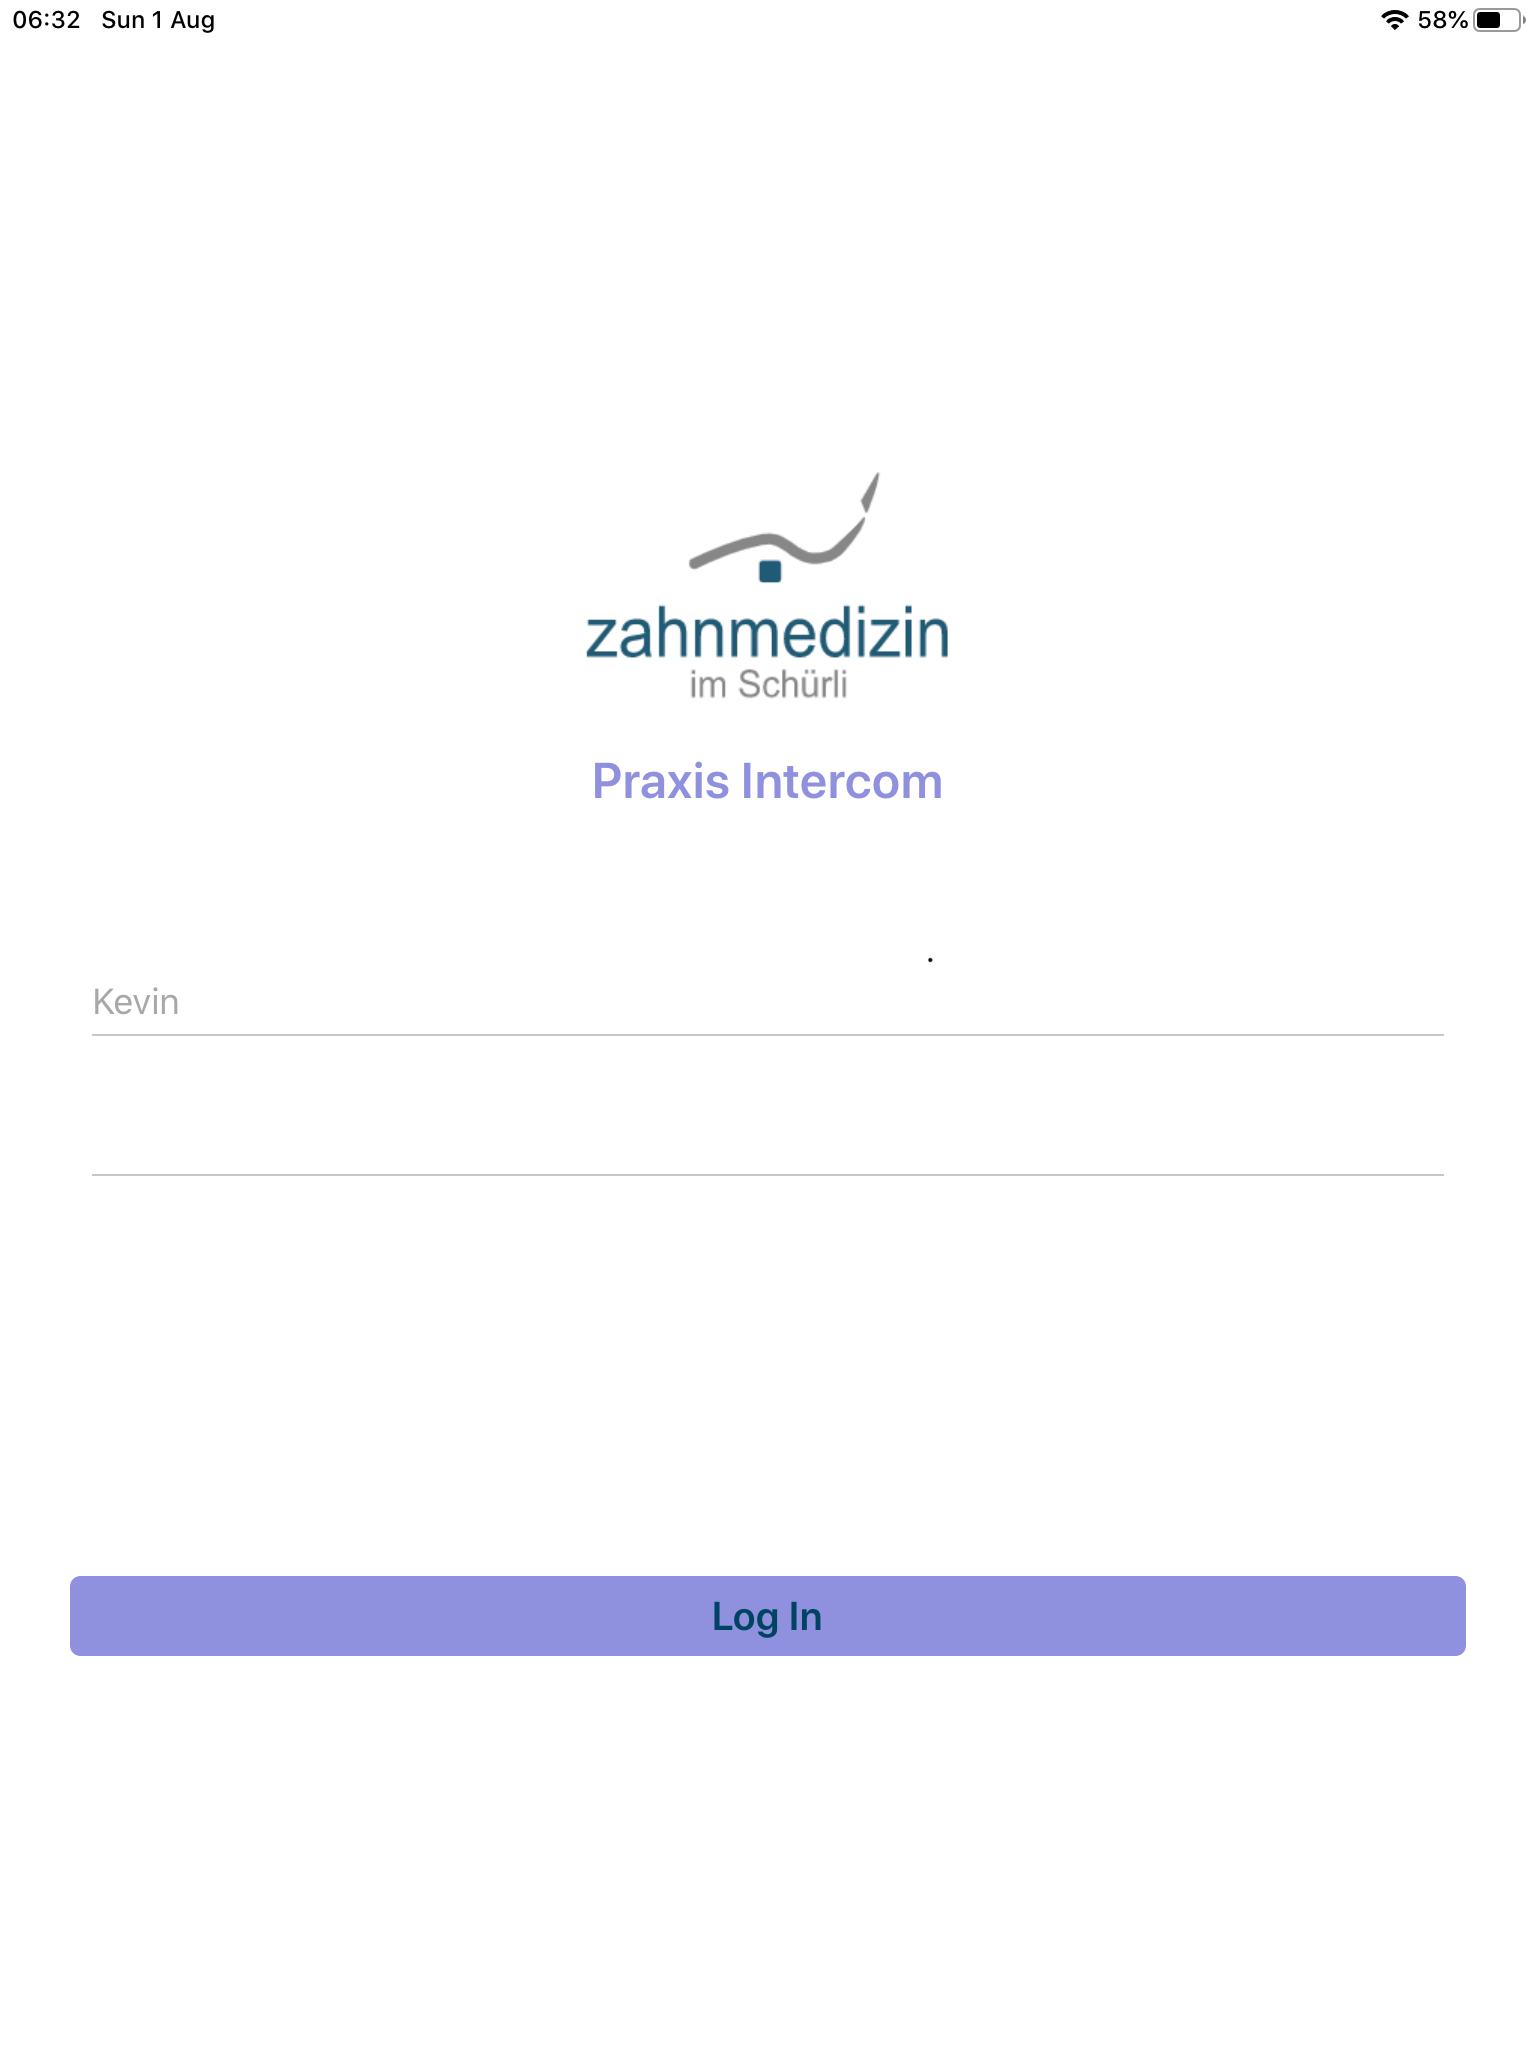
\includegraphics[width=\textwidth]{graphics/screenshots/placeholder}
        \caption{Ansicht Inbox}
    \end{minipage}
    \label{fig:MobileClient-Screens2}
\end{figure}

\clearpage

\subsubsection*{Einstellungen und Aktive Anrufe}

Im Bereich Einstellungen werden Informationen zur gewählten Zimmerkonfiguration und dem angemeldeten Benutzer angezeigt.
Weiter können lokale Einstellungen vorgenommen werden.
Das Vorlesen von empfangenen Benachrichtigungen sowie das Empfangen von Anrufen kann hier deaktiviert werden.
Über einen Button kann der Benutzer sich zudem von der App abmelden.

\begin{figure}[h]
    \centering
    \begin{minipage}[b]{0.4\textwidth}
        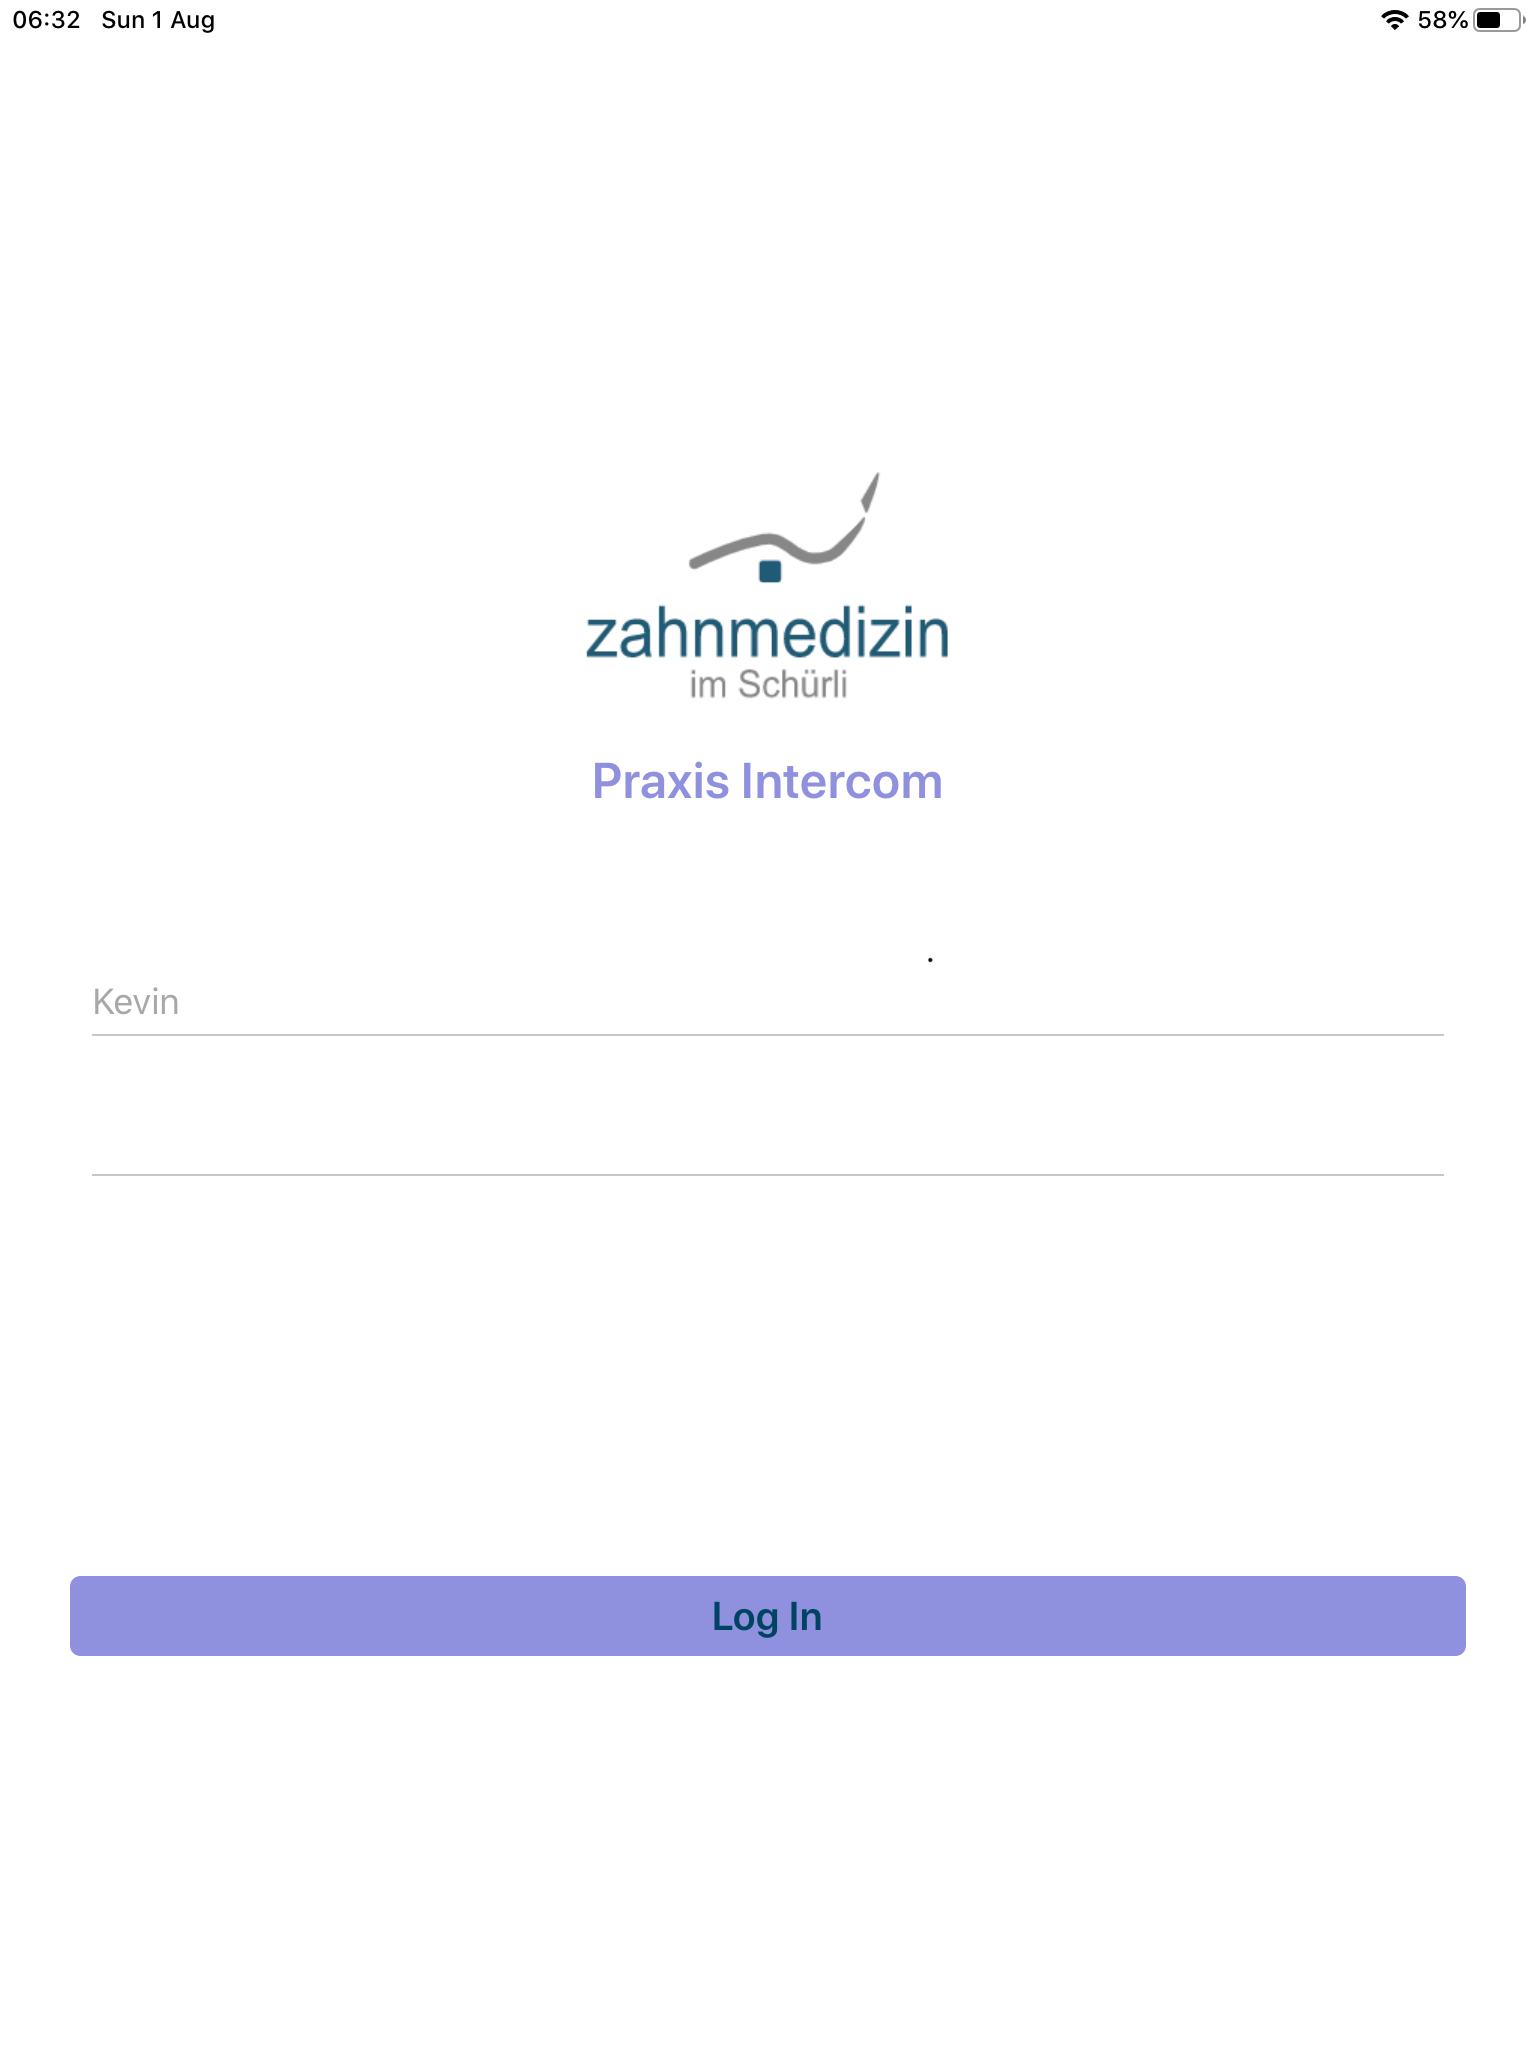
\includegraphics[width=\textwidth]{graphics/screenshots/placeholder}
        \caption{Ansicht Settings}
    \end{minipage}
    \hfill
    \begin{minipage}[b]{0.4\textwidth}
        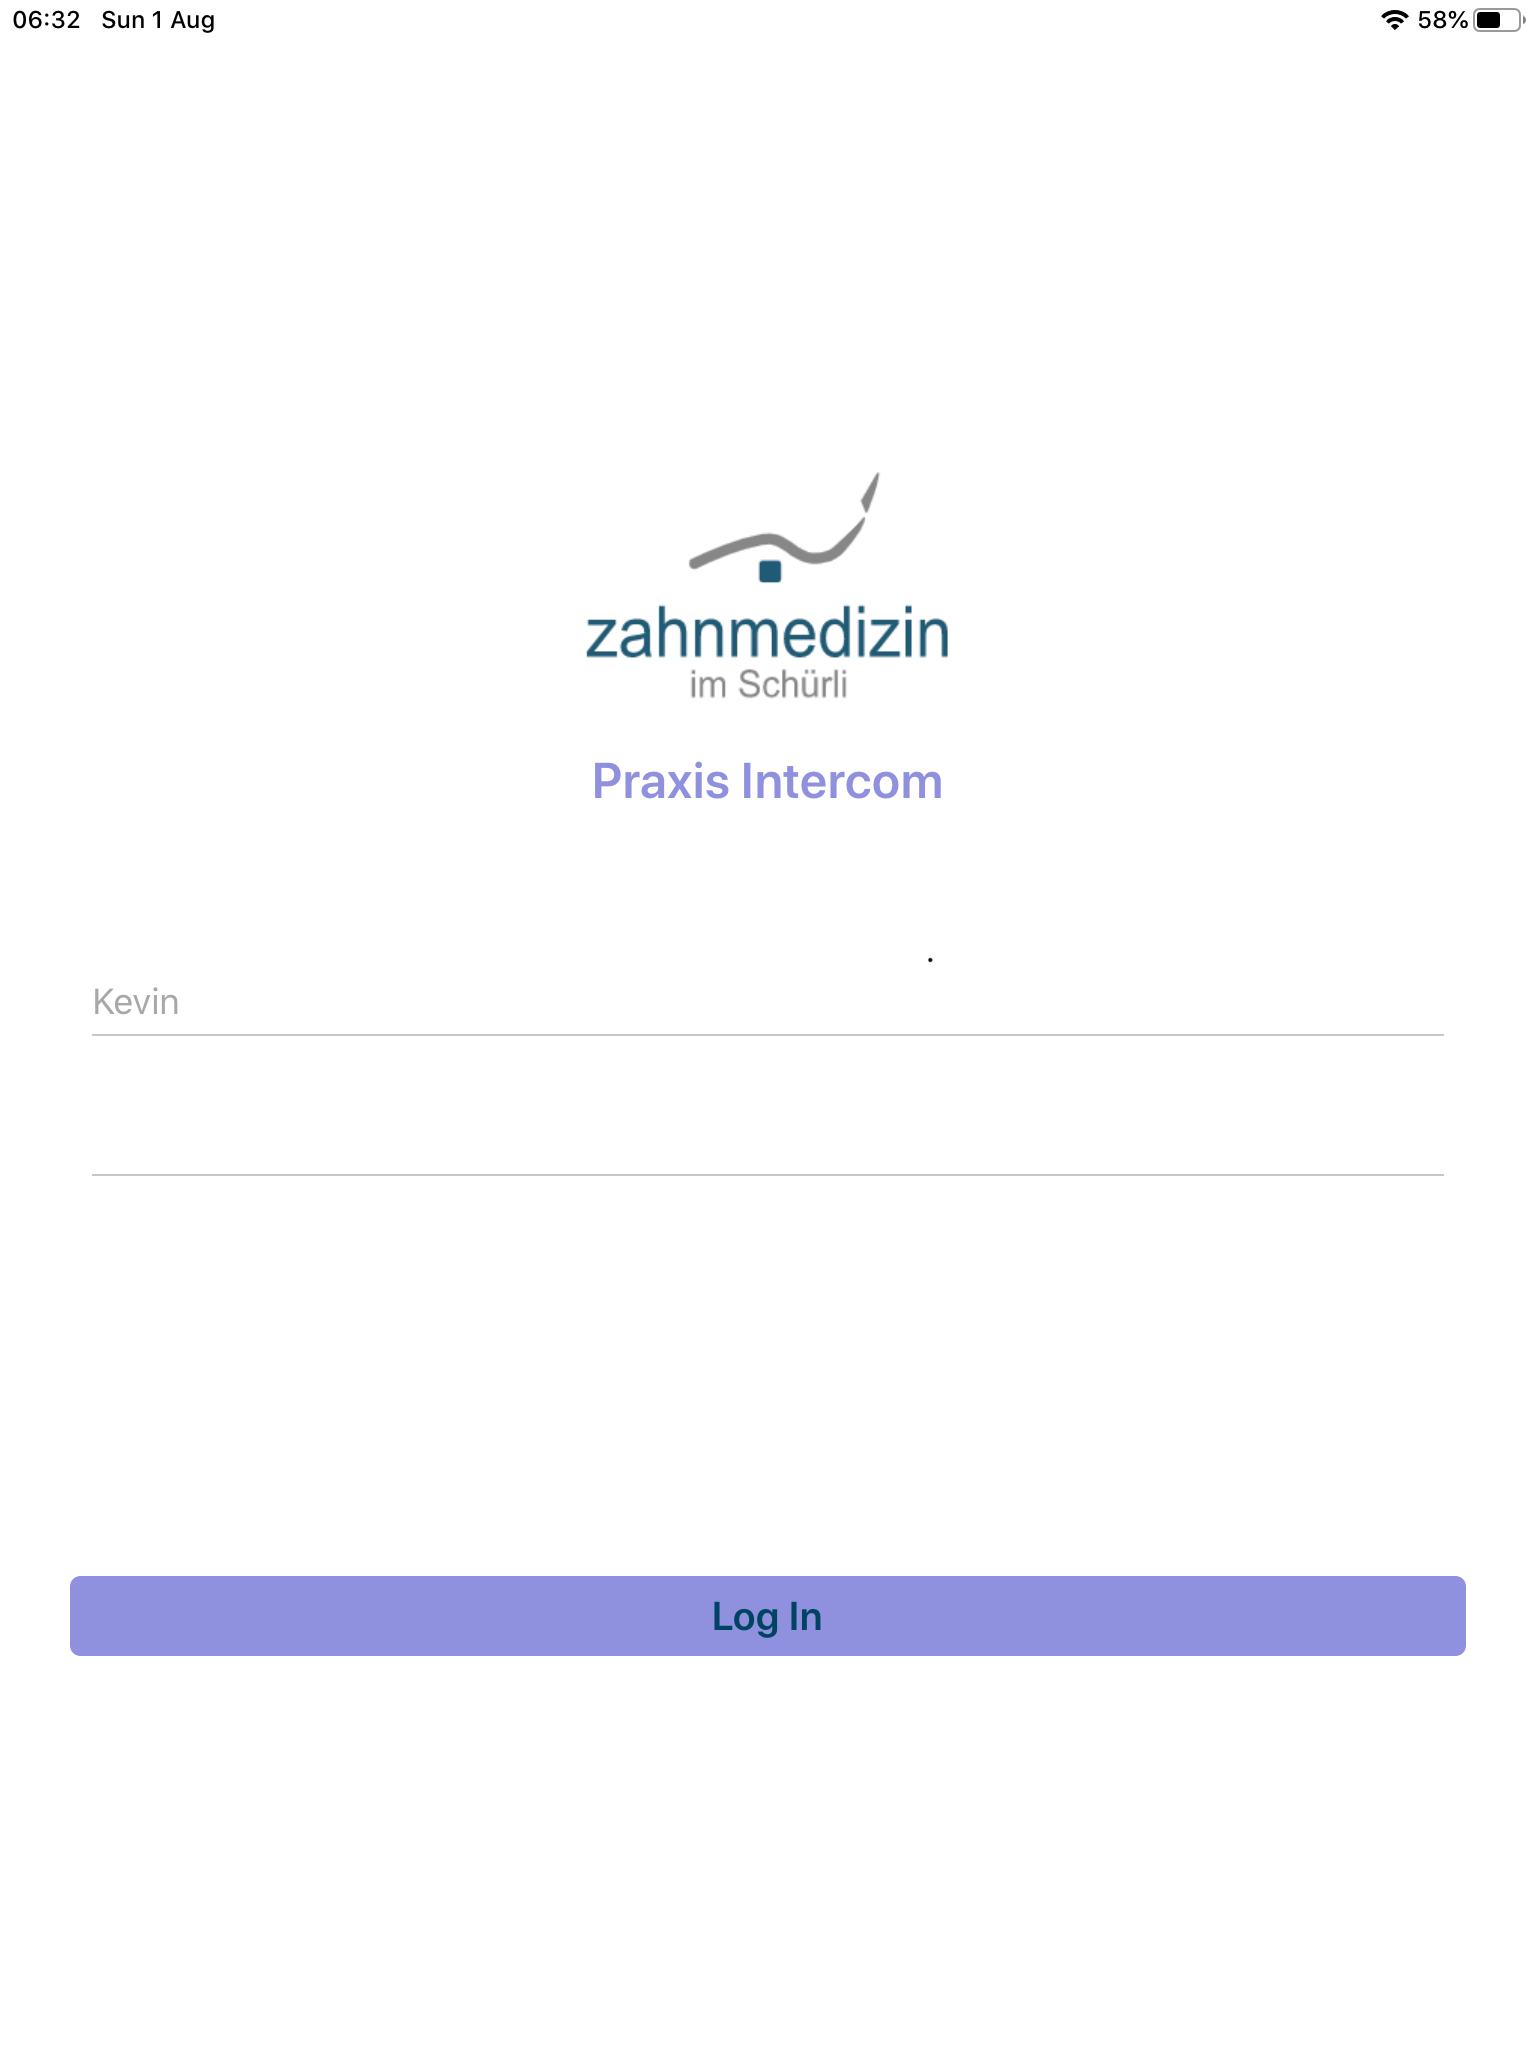
\includegraphics[width=\textwidth]{graphics/screenshots/placeholder}
        \caption{Ansicht Aktiver Anruf}
    \end{minipage}
    \label{fig:MobileClient-Screens3}
\end{figure}

Die Ansicht ''Aktive Anruf'' wird angezeigt, nachdem ein Anruf gestartet wurde.
Entweder, der Anruf durch antippen des Buttons in der Home Ansicht gestartet wurde oder weil ein Anruf von einem anderen Client empfangen wird.
In dieser Ansicht wird der Titel des gestarteten Anrufes bzw. Name des Zimmer des Gesprächspartners angezeigt.
Wenn mehr als ein Gesprächspartner am Anruf beteiligt ist, wird zudem eine Liste der Teilnehmer zusammen mit deren Verbindungsstatus angezeigt.
Allen Gesprächsteilnehmern stehen Buttons zur Stummschaltung des eigenen Lautsprechers und Microphons zur Verfügung.
Zudem können alle Gesprächsteilehmmer die Unterhaltung durch den roten Auflegen Button beenden.

\clearpage

\subsubsection*{Hintergrundbenachrichtigungen und Fehlerhandling}

Das Versenden von Benachrichtigungen ist über die Anbindung des Cloudservices gelöst.
Dieser leitet Benachrichtigungen anhand der Konfiguration über den Messagingservice an die relevanten Empfänger zu.
Bei einem Fehler in der Verarbeitung beim Cloudservice, wird Praxismitarbeitenden direkt mitgeteilt, dass die Benachrichtigung nicht zugestellt werden konnte.
In der App wird ein Dialog angezeigt, welcher darüber informiert und die Möglichkeit bietet, die Aktion direkt zu wiederholen.

\begin{figure}[h]
    \centering
    \begin{minipage}[b]{0.4\textwidth}
        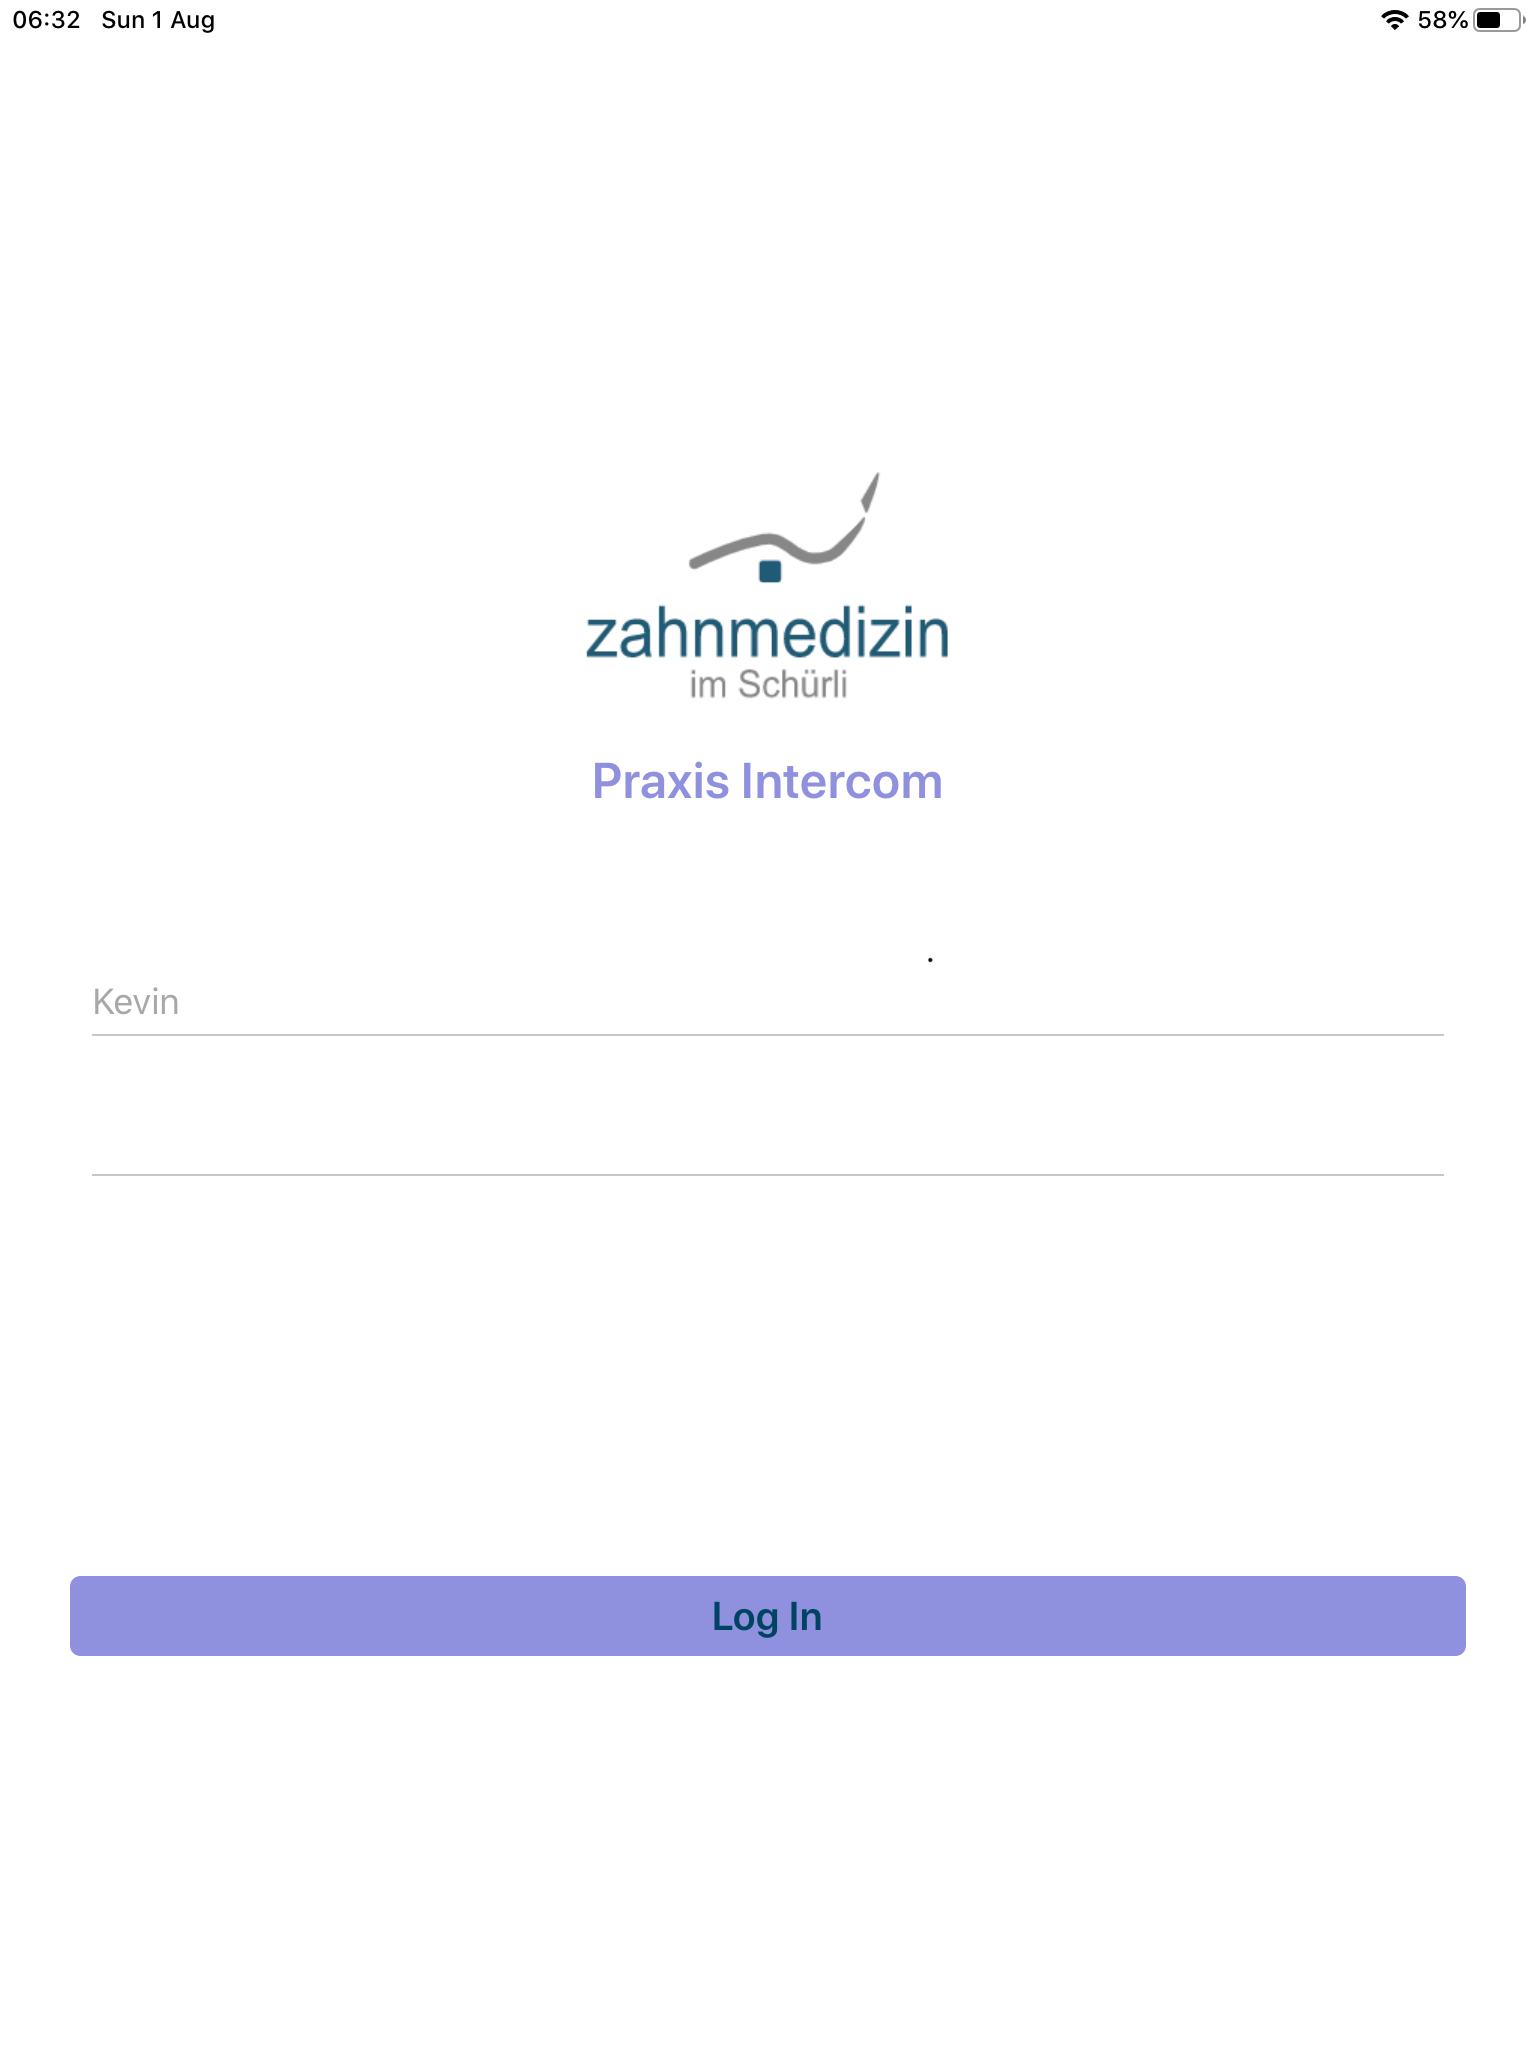
\includegraphics[width=\textwidth]{graphics/screenshots/placeholder}
        \caption{Hintergrund Benachrichtigung}
    \end{minipage}
    \hfill
    \begin{minipage}[b]{0.4\textwidth}
        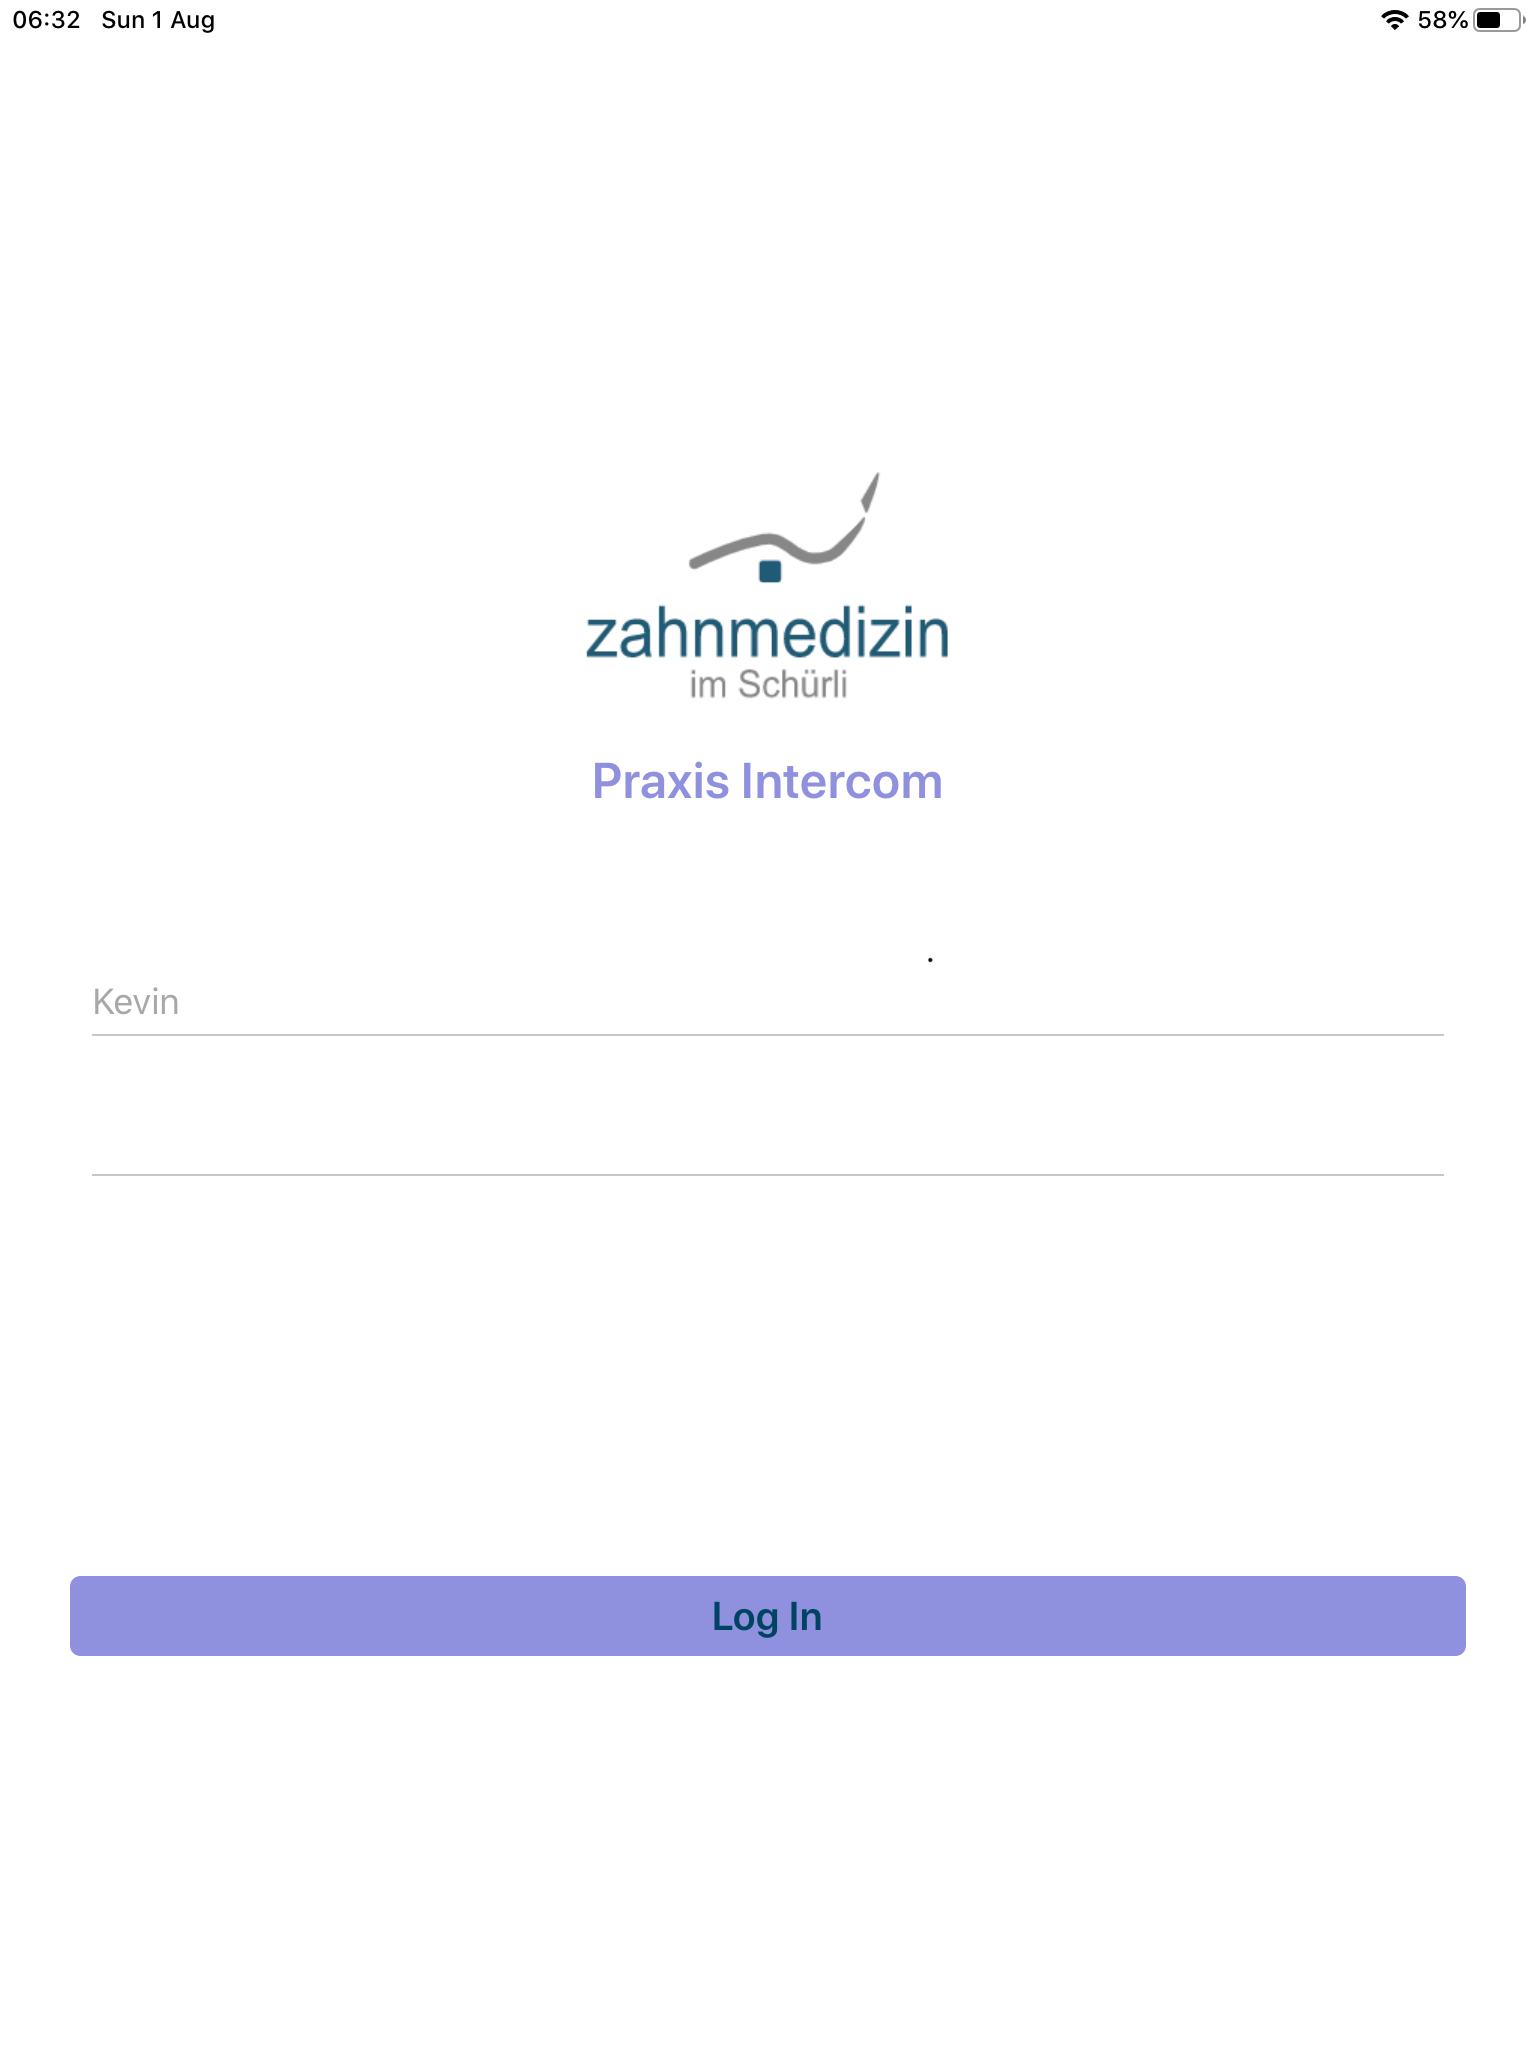
\includegraphics[width=\textwidth]{graphics/screenshots/placeholder}
        \caption{Benachrichtigung wiederholen}
    \end{minipage}
    \label{fig:MobileClient-Screens4}
\end{figure}

Benachrichtigungen können auch im Hintergrund empfangen werden.
Im Hintergrund empfangene Benachrichtigungen erscheinen als Push Benachrichtigungen auf dem Home Screen des iPads.
Anrufe über die Gegensprechanlage können nur empfangen werden, wenn die Applikation geöffnet ist.
Ist die App minimiert oder beendet, ist der jeweilige Client für Gespräche nicht verfügbar.
Ein nicht verfügbarer Client wird über Hintergrundbenachrichtigungen auf verpasste Anrufe hingewiesen.

\clearpage
